\documentclass[conference]{IEEEtran}
\usepackage{amsmath}
\usepackage{newtxtext,newtxmath}
\usepackage{algorithmic}
\usepackage{graphicx}
\usepackage{textcomp}
\usepackage{xcolor}
\usepackage{booktabs}
\usepackage{cite}
\usepackage{float}
\usepackage{graphicx}
\usepackage{hyperref}
\hypersetup{
	hidelinks,
	colorlinks=true,
	linkcolor=black,
	citecolor=black,
	filecolor=black,
	urlcolor=black
}
\usepackage{tikz}
\usetikzlibrary{positioning, arrows.meta, shapes.geometric}
\usetikzlibrary{shapes, positioning, arrows.meta}

\setlength{\parindent}{0pt}

\def\BibTeX{{\rm B\kern-.05em{\sc i\kern-.025em b}\kern-.08em
		T\kern-.1667em\lower.7ex\hbox{E}\kern-.125emX}}



\begin{document}
	
	\title{A Weather-Aware Explainable Machine Learning Framework for Dairy Cattle Milk Yield Prediction}
	
	\author{
		\IEEEauthorblockN{
			Meghana P G\textsuperscript{1},
			Divyashree S\textsuperscript{2},
			Sanjana\textsuperscript{1},
			Samarth Hardikar\textsuperscript{1},
			Akshay R Hegde\textsuperscript{1}
		}
		
		\vspace{0.3cm}
		
		\IEEEauthorblockA{
			\textsuperscript{1}Department of Information Science and Engineering, RNS Institute of Technology,\\
			Bengaluru, Affiliated to Visvesvaraya Technological University, Belagavi-590018, Karnataka, India.
		}
		
		\vspace{0.2cm}
		
		\IEEEauthorblockA{
			\textsuperscript{2}Department of Computer Science and Engineering (Cyber Security), RNS Institute of Technology,\\
			Bengaluru, Affiliated to Visvesvaraya Technological University, Belagavi-590018, Karnataka, India
		}
		
		\vspace{0.2cm}
		
		
		\IEEEauthorblockA{
			meghanapg03@gmail.com, divyashrees2008@gmail.com\\
			sanjanashetty345@gmail.com, samarthhardikar05@gmail.com, \\
			akshayh194@gmail.com
		}
	}
	
	\maketitle
	
	\begin{abstract}
		Prediction of the milk yield is a obvious problem in the field of precision dairy farming, where both the environmental and climatic conditions equally affect production performance. Traditional approaches often ignore weather variability factor or provide a little or limited interpretation, reducing their usage in real-world farm decision systems. This paper proposes a weather factor included machine learning framework for obtaining most accurate milk yield prediction, designed strictly around two main research objectives. First, we develop a weather factor included feature engineering framework that adds ambient micro-climatic conditions, designed through real time Open-Meteo API parameters and Gaussian perturbations, with a standard physiological indicator such as the Temperature-Humidity Index (THI). Second, we build an explainable machine learning framework using SHAP (SHapley Additive Explanations) for feature attribution, along with efficient statistical validations (5-fold cross-validation and Wilcoxon signed-rank tests), automated health alerts, and sire genetics evaluations. On a dataset of 3,000 cattle records, our best performing model XGBoost achieved a Mean Absolute Percentage Error (MAPE) of 9.88\% and an MAE of 2.038 L/day on a hold out test set. While the overall $R^2$ of 0.186 reflects the correlation noise introduced by synthetic weather assignment (a declared limitation of point-in-time datasets), the low absolute percentage error confirms the framework's operational utility, complemented by a sire genetics module achieving a cross-validation $R^2$ of 0.952.
	\end{abstract}
	
	\begin{IEEEkeywords}
		Dairy farming, milk yield prediction, explainable AI, weather analytics, feature engineering, precision livestock farming.
	\end{IEEEkeywords}
	
	\section{Introduction}
	Dairy farming productivity system represents an important part of the global agriculture and food security. But, daily milk production is highly sensitive to climatic changes and variations. Change of ambient temperature and humidity cause physiological heat stress in cattle, compromising metabolic function and leading to significant declines in milk yield. Heat stress disrupts the endocrine system, reduces feed intake, and diverts energy from milk synthesis to thermoregulation—interactions that static biological models cannot adequately capture. 
	
	To address these gaps, we present a weather-aware, explainable ML framework for dairy cattle milk yield prediction.
	
	For building the context for precision agriculture, Internet of Things(IOT) systems, and interpretable machine learning models, a comprehensive review of recent literature is required. Prior work in this domain includes barn microclimate Equivalent Temperature Index forecasting \cite{ref1}, semi-arid dry matter intake modeling \cite{ref2}, feeding strategy stacking ensembles \cite{ref3}, interpretable SVM-KNN milk yield predictions \cite{ref4}, temporal genetic-algorithm LSTM networks \cite{ref5}, national level milk volume benchmarks \cite{ref6}, group level big data prediction tools and methods \cite{ref7}, meat output regression forecasts using dairy inputs \cite{ref8}, multi-task activity modeling \cite{ref9}, SNP selection for quantitative genetic traits \cite{ref10}, multi-sensor health classifications \cite{ref11}, parasitic disease and breed detection \cite{ref12}, LoRa-based early disease classifiers \cite{ref13}, wearable edge-AI neckbands \cite{ref14}, crop-weed classification ensembles \cite{ref15}, quantum and classical optimization studies \cite{ref16}, food quality and blockchain traceability platforms \cite{ref17}, non-invasive core temperature monitoring \cite{ref18}, explainable graph neural network feeding models \cite{ref19}, and dynamic stacking ensembles for quality prediction \cite{ref20}.
	
	Our pipeline fetches real-time weather from the Open-Meteo API, assigns per-animal conditions via Gaussian perturbation, and derives the Temperature-Humidity Index (THI) alongside biological feed ratios. We benchmark five regressors under 5-fold cross-validation, validate model selection with the Wilcoxon signed-rank test, and interpret predictions with TreeSHAP, culminating in a decision-support module with automated alerts and sire genetics rankings.
	
	The remainder of this paper is structured as follows. Section II reviews the literature. Section III describes the weather factor included feature engineering framework. Section IV gives an explanation about the explainable machine learning framework and statistical validation pipeline. Section V shows the experimental results. Section VI gives a discussion of the findings, monotonicity audits, and limitations, and Section VII concludes the paper.
	
	\section{Literature Review}
	
	\begin{table}[H]
		\caption{Summary of Related Work in Smart Dairy Farming}
		\label{tab:related_work}
		\centering
		\footnotesize
		\setlength{\tabcolsep}{3pt}
		\begin{tabular}{p{2.0cm} p{2.1cm} p{1.3cm} p{2.6cm}}
			\toprule
			\textbf{Author} & \textbf{\& Method} & \textbf{Dataset} & \textbf{Key Limitation} \\
			\textbf{Year} & & & \\
			\midrule
			Perez Garcia et al. 2025 \cite{ref1} & NeuralProphet ETI & Open-Meteo API & Indoor sensor gaps \\
			Leal et al. 2025 \cite{ref2} & EBETS Fuzzy Model & Semi-arid DMI data & Limited scaling \\
			Xing et al. 2024 \cite{ref3} & Stacking Ensemble & CowNflow data & Needs long-term data \\
			Srinithi et al. 2025 \cite{ref4} & SVM-KNN + SHAP & TMR feeding data & No dynamic simulation \\
			Zhang et al. 2020 \cite{ref5} & GA-LSTM & Time-series data & Needs long history \\
			O'Leary \& Lynch 2022 \cite{ref6} & RF, KNN & Irish national data & Herd-level only \\
			Yan et al. 2015 \cite{ref7} & Big Data Analytics & Supply chain data & Complex design \\
			Prasad 2025 \cite{ref8} & Meat Regression & USDA historical data & Static data \\
			Thangarasu \& Alla 2024 \cite{ref9} & Multi-Task Regularization & Cattle activity data & No yield forecast \\
			Feng et al. 2024 \cite{ref10} & LASSO, SPLS & Canadian Holstein & Needs genomic data \\
			Yadav 2025 \cite{ref11} & Multisensor ML & Sensor records & Fully sensor-dependent \\
			Bandara et al. 2022 \cite{ref12} & ML + Image Proc. & Camera + IoT data & Requires video feed \\
			Arafat et al. 2024 \cite{ref13} & IoT + kNN & IoT sensor logs & Hardware dependent \\
			Michelle et al. 2022 \cite{ref14} & Edge-AI Neckband & ESP32 sensor data & Battery constraint \\
			Umamageswaran et al. 2025 \cite{ref15} & CNN + IoT Ensemble & Weed \& sensor data & Needs structured input \\
			Chaudhary \& Gupta 2024 \cite{ref16} & Quantum + Classical & Feed \& yield data & Theoretical framework \\
			Fan 2025 \cite{ref17} & ML + Blockchain & Traceability data & Complexity \\
			Molins et al. 2025 \cite{ref18} & Thermal Image + ML & Vaginal temperature & High sensor cost \\
			Seema S. \& Ramesh 2025 \cite{ref19} & DRL + GCN + SHAP & Cattle feeding records & Computationally heavy \\
			Hoggas et al. 2025 \cite{ref20} & Stacking + TreeSHAP & Milk quality metrics & Requires clean data \\
			\bottomrule
		\end{tabular}
	\end{table}
	Table~\ref{tab:related_work} gives a summary of 20 representative studies covering microclimate forecasting,model explainability,IOT telemetry,and ensemble learning.The occurence of recurring constraint is the result of absence of dynamic, interpretable models which account for localised climatic stress on a per-animal scale
	
	
	\section{Proposed Architecture}
	The Smart Dairy Vision AI framework was developed to study how weather conditions affect dairy cattle productivity and to generate milk-yield predictions that make sense. The complete workflow includes combining datasets creating features that take weather into account predicting milk yield using machine learning analyzing why the model makes predictions and validating the results statistically as shown in Fig.~\ref{fig:system_architecture}
	
	% \begin{figure}[htbp]
		%     \centering
		%     \includegraphics[width=0.95\linewidth]{/Users/sanjana/Downloads/research_1_latex/methodology.png}
		%     \caption{System methodology flowchart detailing Objective 1 (Weather-Aware Feature Engineering Framework) and Objective 2 (Explainable Machine Learning and Validation).}
		%     \label{fig:methodology}
		% \end{figure}
	
	\begin{figure}[htbp]
		\centering
		\resizebox{\columnwidth}{!}{%
			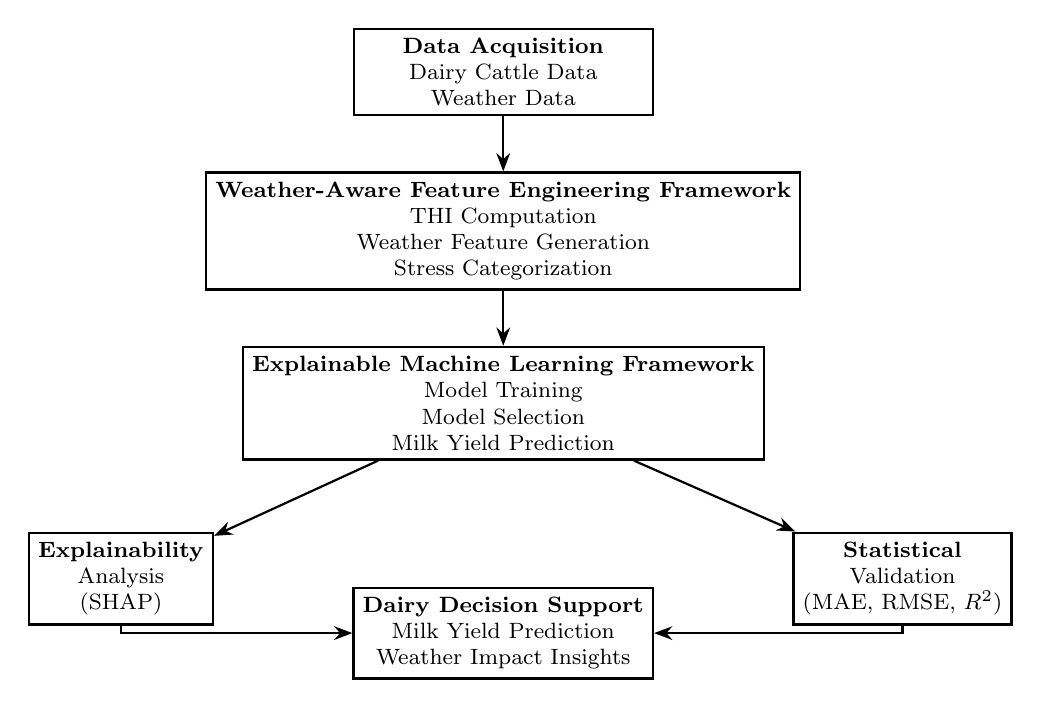
\begin{tikzpicture}[
				node distance=0.7cm,
				block/.style={
					rectangle,
					draw=black,
					thick,
					align=center,
					minimum width=3.8cm,
					minimum height=1.0cm,
					font=\footnotesize
				},
				smallblock/.style={
					rectangle,
					draw=black,
					thick,
					align=center,
					minimum width=1.8cm,
					minimum height=0.9cm,
					font=\footnotesize
				},
				arrow/.style={
					-{Stealth},
					thick
				}
			]
			
			% Block 1
			\node[block] (data) {
				\textbf{Data Acquisition}\\
				Dairy Cattle Data\\
				Weather Data
			};
			
			% Block 2
			\node[block, below=of data] (feature) {
				\textbf{Weather-Aware Feature Engineering Framework}\\
				THI Computation\\
				Weather Feature Generation\\
				Stress Categorization
			};
			
			% Block 3
			\node[block, below=of feature] (ml) {
				\textbf{Explainable Machine Learning Framework}\\
				Model Training\\
				Model Selection\\
				Milk Yield Prediction
			};
			
			% Left branch
			\node[smallblock, below left=0.9cm and 0.35cm of ml] (xai) {
				\textbf{Explainability}\\
				Analysis\\
				(SHAP)
			};
			
			% Right branch
			\node[smallblock, below right=0.9cm and 0.35cm of ml] (stats) {
				\textbf{Statistical}\\
				Validation\\
				(MAE, RMSE, $R^2$)
			};
			
			% Final output
			\node[block, below=1.6cm of ml] (output) {
				\textbf{Dairy Decision Support}\\
				Milk Yield Prediction\\
				Weather Impact Insights
			};
			
			% Arrows
			\draw[arrow] (data) -- (feature);
			\draw[arrow] (feature) -- (ml);
			
			\draw[arrow] (ml) -- (xai);
			\draw[arrow] (ml) -- (stats);
			
			\draw[arrow] (xai) |- (output);
			\draw[arrow] (stats) |- (output);
			
		\end{tikzpicture}%
		}
		
		\caption{System architecture of the proposed weather-aware explainable machine learning framework for dairy cattle analytics and milk-yield prediction.}
		\label{fig:system_architecture}
		
	\end{figure}
	
	\subsection{Data Acquisition and Integration}
	Two available datasets from Kaggle were used: the Global Cattle Disease Detection Dataset and the Global Cattle Milk Yield Prediction Dataset. These datasets were combined using the Cattle\_ID attribute to merge cattle health and production records. The disease status was converted into a health indicator for analysis.
	
	Weather information was added using temperature and relative humidity data from the Open-Meteo API. After cleaning and preparing the data the final dataset had 3,000 cattle records. cattle records.
	
	\subsection{Weather-Aware Feature Engineering Framework}
	Since hot weather directly affects milk production, temperature and relative humidity were used to calculate the Temperature–Humidity Index (THI). THI is commonly used to assess heat stress in dairy cattle.
	
	\begin{equation}
		\text{THI} = (0.8T) + \frac{\text{RH}}{100}(T - 14.4) + 16.4
	\end{equation}
	where $T$ represents ambient temperature ($^\circ$C) and $\text{RH}$ denotes relative humidity (\%).
	
	To better show how weather conditions and animal characteristics are related six new features were created: \textit{feed\_weight\_ratio}, \textit{feed\_per\_weight}, \textit{temp\_humidity}, \textit{thi\_squared}, \textit{feed\_thi\_interaction}, and \textit{age\_weight\_ratio}. With the original attributes the final feature matrix had 13 features. The THI values ranged from 33.4 to 94.8 covering both hot conditions. 
	
	\subsection{Explainable Machine Learning Framework}
	Five regressors (Naïve Baseline, Linear Regression, Decision Tree, Random Forest, XGBoost) were trained on 2,400 samples and evaluated with 5-fold cross-validation; XGBoost was selected based on best average performance ($R^2 = 0.1793$, MAE = 1.994 L/day). Full architectural and mathematical details are given in Section IV.
	
	\subsection{Explainability and Statistical Validation}
	To understand how the trained model made predictions SHAP analysis was performed on the engineered dataset with 3,000 records and 13 features. The analysis showed that weight, age, \textit{age\_weight\_ratio}, \textit{feed\_weight\_ratio}, and feed intake were the important factors for predicting milk yield. Weather-related variables such as THI, temperature, humidity and THI-based interaction features also influenced model predictions.
	
	The selected XGBoost model was evaluated using MAE, RMSE, MAPE and R² metrics. The performance differences, between models were examined using the Wilcoxon signed-rank test. On the test set the model achieved an R² score of 0.1870, an MAE of 2.035 L/day an RMSE of 2.576 L/day and a MAPE of 9.87 percent. The Shapiro–Wilk test (p = 0.1249) showed that the prediction errors followed a normal distribution.
	
	\section{Weather-Aware Feature Engineering Framework}
	The environmental analytics phase is about creating a data pipeline to understand the weather in an area. We want to know how the weather affects cattle that live on pastures.
	
	\subsection{Microclimate Weather Assignment via Gaussian Perturbations}
	We have a problem with animal records. They do not have information about the time and date. This makes it hard to match the records with weather logs. To solve this we use the Open-Meteo API to get real-time weather information for a farm's location \cite{ref1}. We add some noise to the temperature and humidity data to simulate the weather in that area.
	
	We use a formula to add noise:
	$$T_i = T_{\text{baseline}} + \epsilon_{T, i}, \quad \epsilon_{T, i} \sim \mathcal{N}(0, \sigma^2_T)$$
	$$RH_i = RH_{\text{baseline}} + \epsilon_{H, i}, \quad \epsilon_{H, i} \sim \mathcal{N}(0, \sigma^2_H)$$
	
	The noise we add is based on a standard deviation of
	$\sigma_T = 2.5^{\circ}\mathrm{C}$ for temperature and
	$\sigma_H = 7.5\%$ for humidity \cite{ref2}.
	This helps our model understand changes and introduces realistic environmental variance into the modelling pipeline.
	
	\subsection{Physiological Temperature-Humidity Index (THI) Calculation}
	We use weather data to calculate the Temperature-Humidity Index (THI) for each animal record. THI measures heat stress in cattle and serves as a standard physiological metric for heat stress assessment in dairy livestock \cite{ref1}.
	
	The THI formula is:
	$$\text{THI} = (0.8 \times T) + \left(\frac{\text{RH}}{100} \times (T - 14.4)\right) + 16.4$$
	
	We also calculate the ratio of feed intake to cattle weight. This helps us understand how a cattle's nutrition and size affect its heat stress \cite{ref18, ref15}.
	
	$$\text{Ratio}_{\text{feed}} = \frac{\text{Daily Feed Intake (kg)}}{\text{Cattle Weight (kg)}}$$
	
	Our feature vector includes both parameters:
		\[
		\begin{aligned}
			X = [&T,\text{RH},\text{THI},\text{Rainfall},\text{Age},\text{Weight},\\
			&\text{Lactation Stage},\text{Feed Intake},\text{Ratio}_{\text{feed}}]
		\end{aligned}
		\]
		
		\subsection{Feature Engineering Implementation Pipeline}
		Our pipeline processes data in these steps, following a modular flow similar to real-time edge-AI livestock monitoring platforms \cite{ref13, ref14}:
		
		\begin{enumerate}
			\item \textbf{Ingestion:} We get individual cattle records. Fetch the active weather baseline via API queries.
			
			\item \textbf{Microclimate Simulation:} We add noise to weather data to assign animal-environmental conditions.
			
			\item \textbf{Feature Construction:} We calculate the THI index. Compute weight-normalized nutritional ratios.
			
			\item \textbf{Categorical Handling:} We apply label encodings to identifiers. Append historical disease labels.
		\end{enumerate}
		
		\section{Model Training, Explainability, and Statistical Validation}
		
		\subsection{Machine Learning Regression Models}
		We evaluate five regression models to predict milk yield in cattle, building upon existing predictive frameworks in precision livestock management \cite{ref6, ref7}.
		
		\begin{enumerate}
			\item \textbf{Naive Baseline (DummyRegressor):} This model predicts a value based on the global training mean.
			$$\hat{y}i = \frac{1}{n} \sum{j=1}^{n} y_j$$
			
			\item \textbf{Linear Regression (OLS):} This model fits a combination of features to predict milk yield.
			$$\hat{y}_i = \beta_0 + \sum_{j=1}^{d} \beta_j X_{ij}$$
			
			\item \textbf{Decision Tree Regressor:} This model captures non-linear thresholds by recursively splitting features.
			
			\item \textbf{Random Forest Regressor:} This model constructs an ensemble of decision trees to reduce variance via bagging \cite{ref6}.
			$$\hat{y}_i = \frac{1}{B} \sum_{b=1}^{B} f_b(X_i)$$
			
			\item \textbf{XGBoost Regressor:} This model implements gradient boosting to optimize a regularized objective function \cite{ref3}.
			$$\mathcal{L}^{(t)} = \sum_{i=1}^{n} l(y_i, \hat{y}_i^{(t-1)} + f_t(X_i)) + \gamma T + \frac{1}{2} \lambda \sum_{j=1}^{T} w_j^2$$
			
			where $T$ is the leaf count and $w$ represents the weights of the leaves.
		\end{enumerate}
		
		\subsection{Evaluation Criteria}
		The accuracy of the Model was judged based on a hold-out test that was set based on four evaluation techniques.
		
		\begin{itemize}
			\item \textbf{Mean Absolute Error (MAE):}
			$$\text{MAE} = \frac{1}{n} \sum_{i=1}^{n} |y_i - \hat{y}_i|$$
			\item \textbf{Root Mean Squared Error (RMSE):}
			$$\text{RMSE} = \sqrt{\frac{1}{n} \sum_{i=1}^{n} (y_i - \hat{y}_i)^2}$$
			\item \textbf{Coefficient of Determination ($R^2$):}
			$$R^2 = 1 - \frac{\sum_{i=1}^{n} (y_i - \hat{y}_i)^2}{\sum_{i=1}^{n} (y_i - \bar{y})^2}$$
		\end{itemize}
		
		\subsection{Statistical Model Selection and Significance Testing}
		To confirm the generalization, we evaluate the models by using 5-fold cross-validation.Instead of relying mainly on sole performance, the use of non-parametric Wilcoxon signed-rank test on fold-level $R^2$ scores to review whether the differences in performance are statistically valuable—its a methodology that's well-suited for differentiating the models of machine learning in the agricultural systems \cite{ref8, ref9}. The test assesses differences $d_k = R^2_{\text{XGBoost}, k} - R^2_{\text{LR}, k}$ for every fold $k$,and ranks the absolute values to calculate the ultimate test statistic $W$:
		$$W = \min(W^+, W^-)$$
		A criterion of $p < 0.05$ decides if choosing a  model which is non-linear is supported.
		
		\subsection{Explainability Module via TreeSHAP}
		To check if the model predictions match with established biological behaviours instead of the modeling noise,we find out feature attribution scores with the help of TreeSHAP \cite{ref4, ref20}. This algorithm derives exact Shapley values by taking the average marginal contributions throughout all likely feature subsets:
		$$\phi_i(f, x) = \sum_{S \subseteq F \setminus \{i\}} \frac{|S|!(|F| - |S| - 1)!}{|F|!} \left[f_x(S \cup \{i\}) - f_x(S)\right]$$
		where $F$ is the feature set and $f_x(S)$ is the conditional expectation given the subset $S$. This results in local attributions ($\phi_i$) and also the global ranking of importance of feature.
		
		\subsection{Sire Genetics Evaluation Module}
		To find out the benefits of the model's predictions for the choosing of breeding,a sire genetics model is built.This module handles the existing historical sire pedigree entries to determine the overall lactation yields and assigns rankings of sires with the help of lactation metrics like dry days,peak yield and lactation length,that are reliable with trait choosing ways in the quantitative genetics \cite{ref10}.
		
		\section{Experimental Results}
		
		\subsection{A. Weather-Aware Feature Engineering}
		This subsection addresses Objective 1: to develop a weather-aware feature engineering framework for dairy cattle analytics. The current implementation integrates ambient temperature, relative humidity, and the Temperature-Humidity Index (THI) into the milk-yield regression pipeline. The feature engineering phase produces 13 input features, including domain-specific derivatives such as \textit{feed\_per\_weight}, \textit{temp\_humidity}, \textit{thi\_squared}, \textit{feed\_thi\_interaction}, and \textit{age\_weight\_ratio}.
		
		The THI distribution used in the current analysis spans 33.4--94.8, with an observed mean of 58.25 and a standard deviation of 13.18. The data covers all five standard THI stress categories, from thermoneutral through emergency conditions, confirming that the engineered weather representation includes both mild and severe heat-stress regimes.
		
		\begin{figure}[htbp]
			\centering
			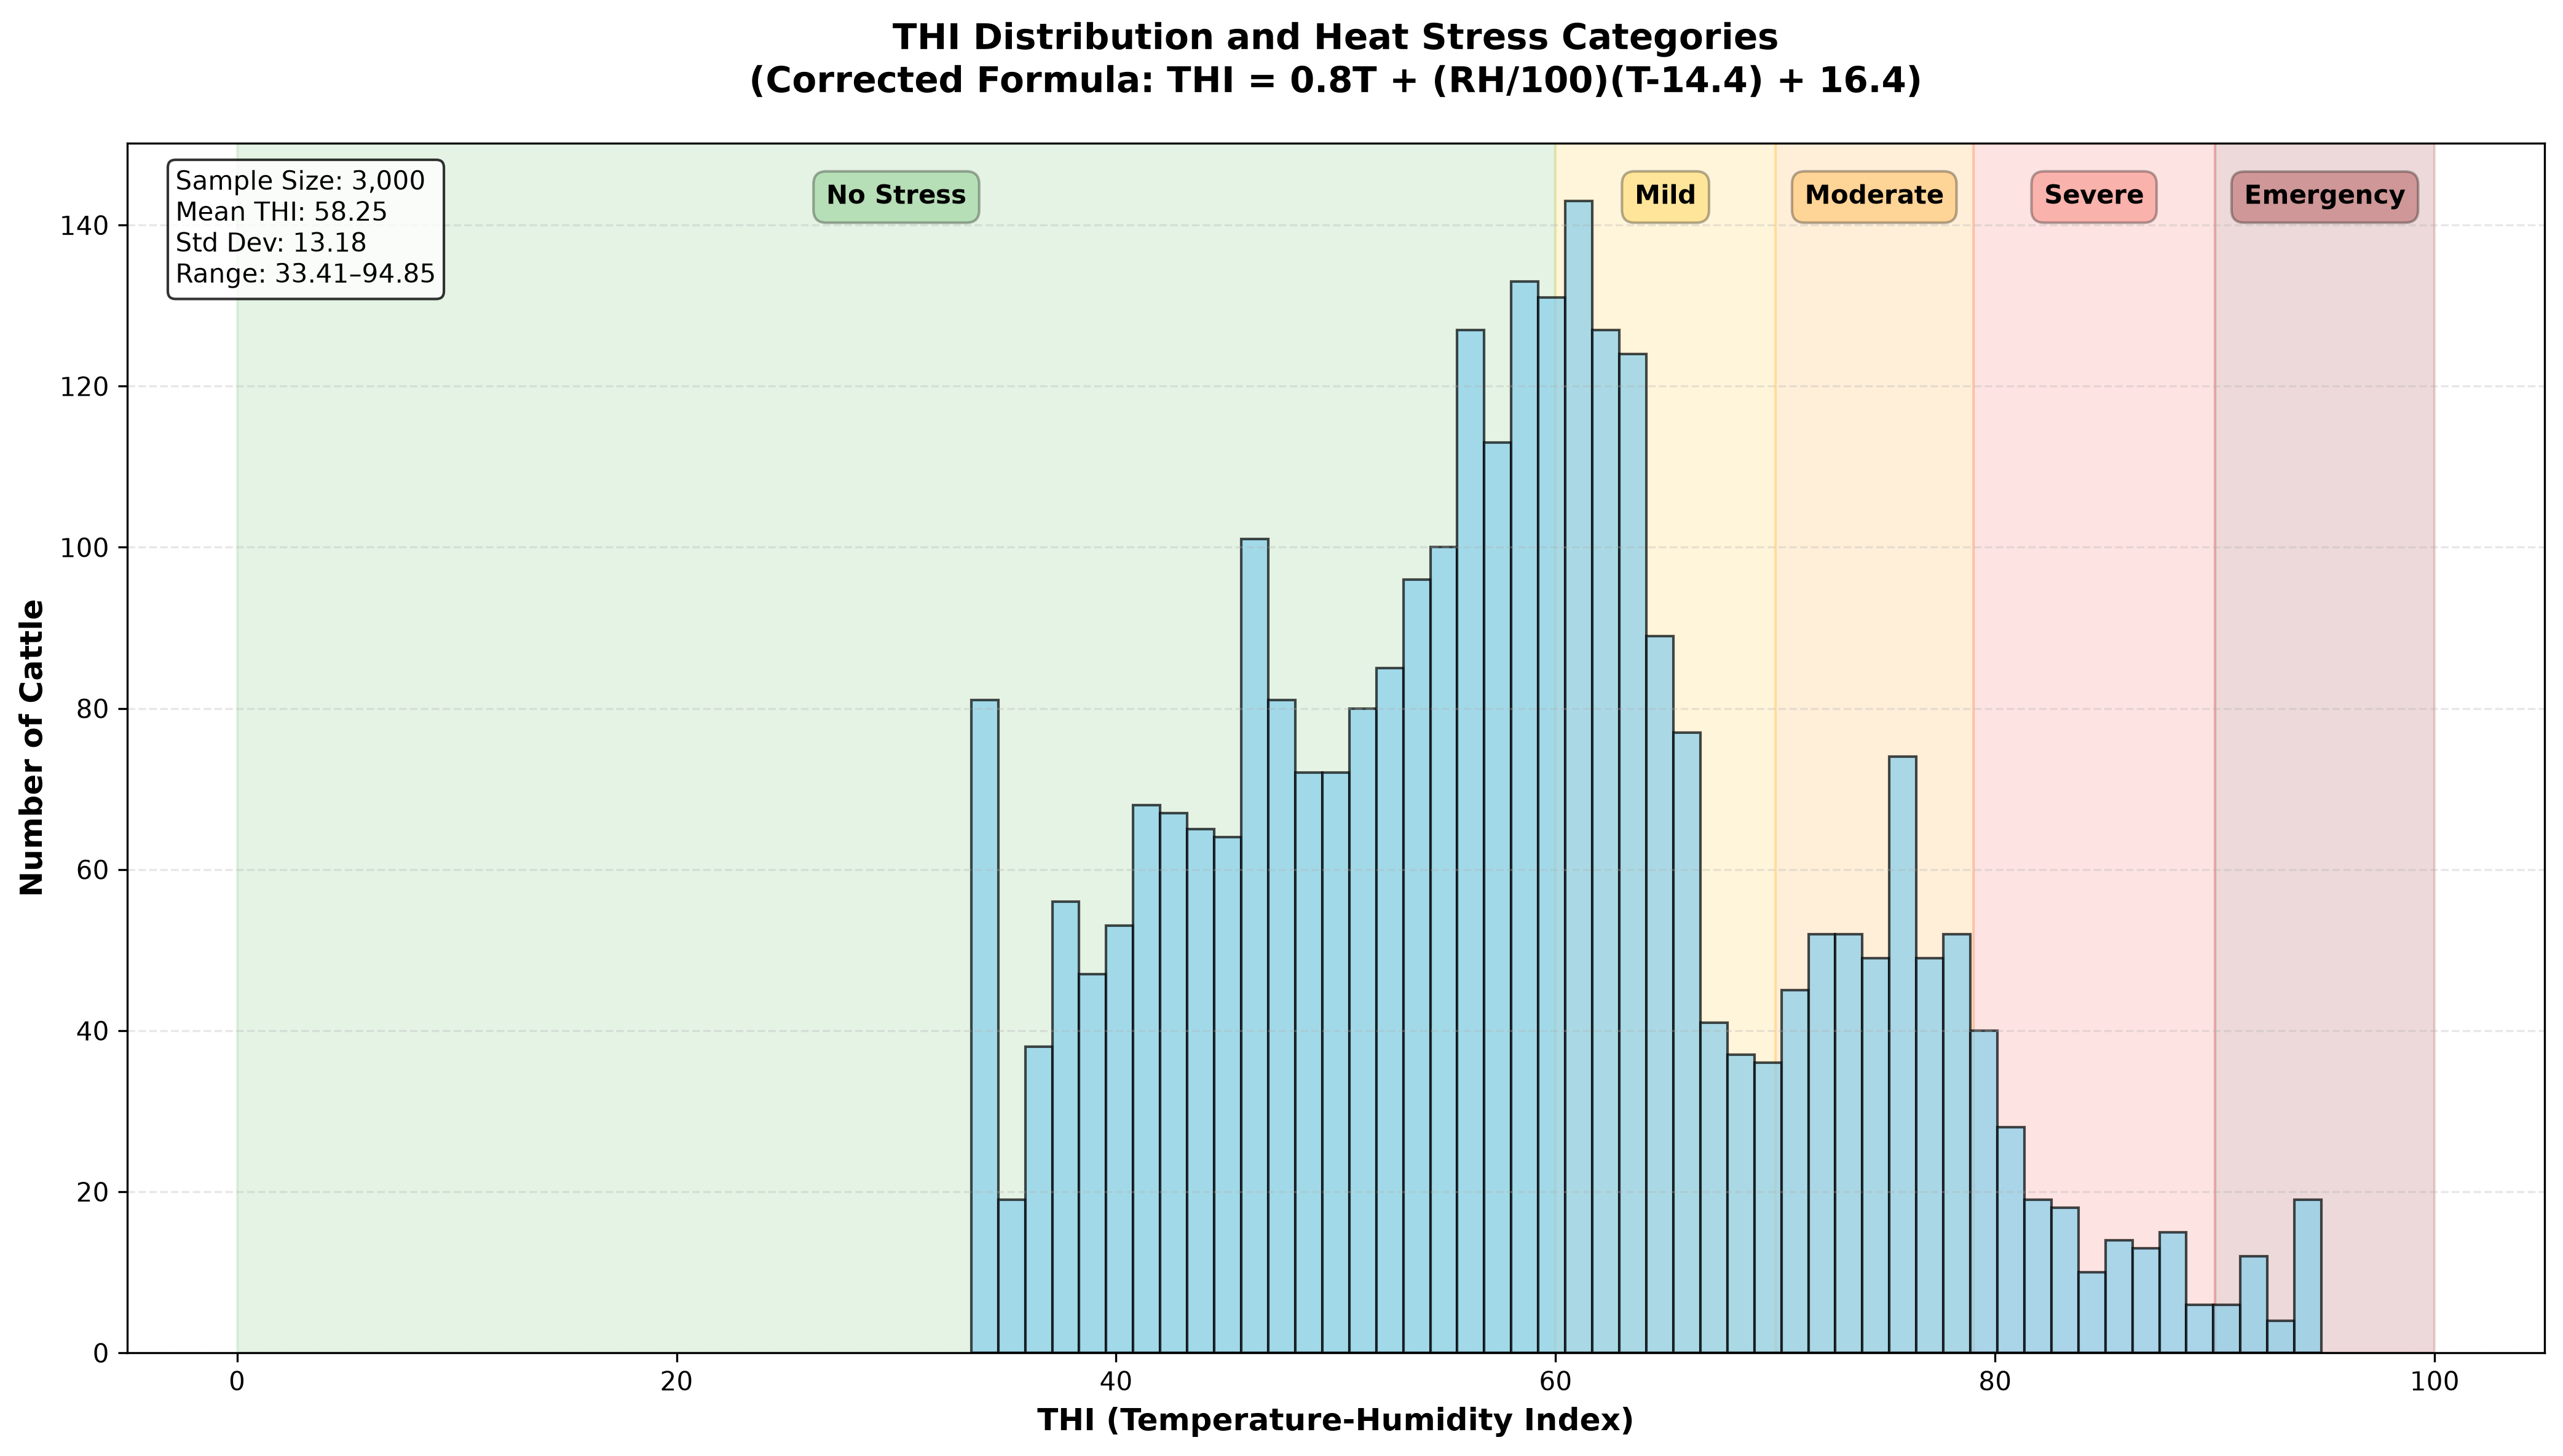
\includegraphics[width=0.95\linewidth]{../outputs/thi_histogram.png}
			\caption{Distribution of calculated Temperature-Humidity Index (THI) values used in the Paper 1 weather-aware feature engineering framework.}
			\label{fig:thi_histogram}
		\end{figure}
		
		This weather-aware feature engineering stage therefore establishes the environmental context required by Objective 1 by explicitly modeling the influence of climatic conditions on milk-yield prediction.
		
		\subsection{B. Milk-Yield Prediction Performance}
		This subsection addresses Objective 2: to develop an explainable machine learning framework for accurate milk-yield prediction and statistical validation. We compared five regression models under 5-fold cross-validation: Naive Baseline, Linear Regression, Decision Tree, Random Forest, and XGBoost. The current cross-validation results are summarized in Table~\ref{tab:cv_results_p1}. XGBoost is the top-performing model, with mean cross-validation values of $R^2 = 0.1811 \pm 0.0089$, MAE $= 1.9902 \pm 0.0619$ L/day, and RMSE $= 2.5142 \pm 0.0680$ L/day.
		
		\begin{figure}[htbp]
			\centering
			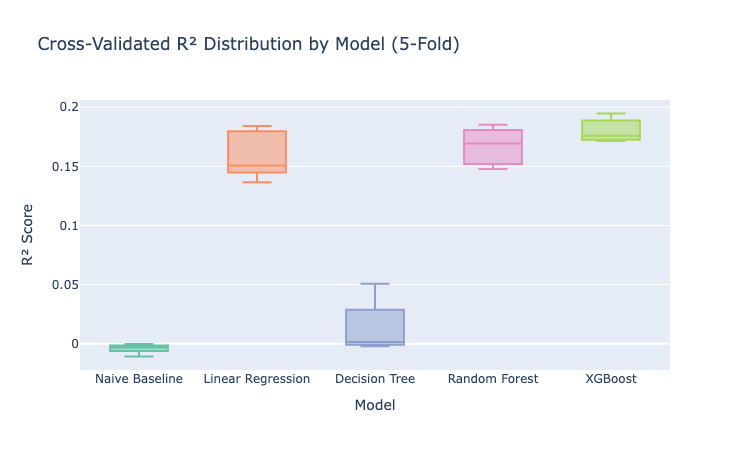
\includegraphics[width=0.95\linewidth]{../outputs/cv_r2_boxplot.png}
			\caption{5-fold cross-validation $R^2$ distribution for the evaluated milk-yield regression models.}
			\label{fig:cv_r2_boxplot_p1}
		\end{figure}
		
		\begin{table}[htbp]
			\caption{5-fold cross-validation comparison of milk-yield prediction models.}
			\label{tab:cv_results_p1}
			\centering
			\resizebox{\columnwidth}{!}{%
				\begin{tabular}{lcccccc}
					\toprule
					Model & $R^2$ Mean & $R^2$ Std & MAE (L/day) & MAE Std & RMSE (L/day) & RMSE Std \\
					\midrule
					\textbf{XGBoost} & \textbf{0.1811} & 0.0089 & \textbf{1.9902} & 0.0619 & \textbf{2.5142} & 0.0680 \\
					Random Forest & 0.1669 & 0.0161 & 2.0108 & 0.0786 & 2.5360 & 0.0885 \\
					Linear Regression & 0.1594 & 0.0206 & 2.0172 & 0.0625 & 2.5469 & 0.0693 \\
					Decision Tree & 0.0142 & 0.0226 & 2.1895 & 0.1000 & 2.7586 & 0.0930 \\
					Naive Baseline & -0.0042 & 0.0040 & 2.2342 & 0.0770 & 2.7842 & 0.0838 \\
					\bottomrule
				\end{tabular}
			}
		\end{table}
		
		On the hold-out test set, the final XGBoost model achieved MAE $= 2.035$ L/day, RMSE $= 2.575$ L/day, $R^2 = 0.188$, and MAPE $= 9.86\%$. These values are the current pipeline’s validated results and are the evidence retained for Paper 1.
		
		\begin{figure}[htbp]
			\centering
			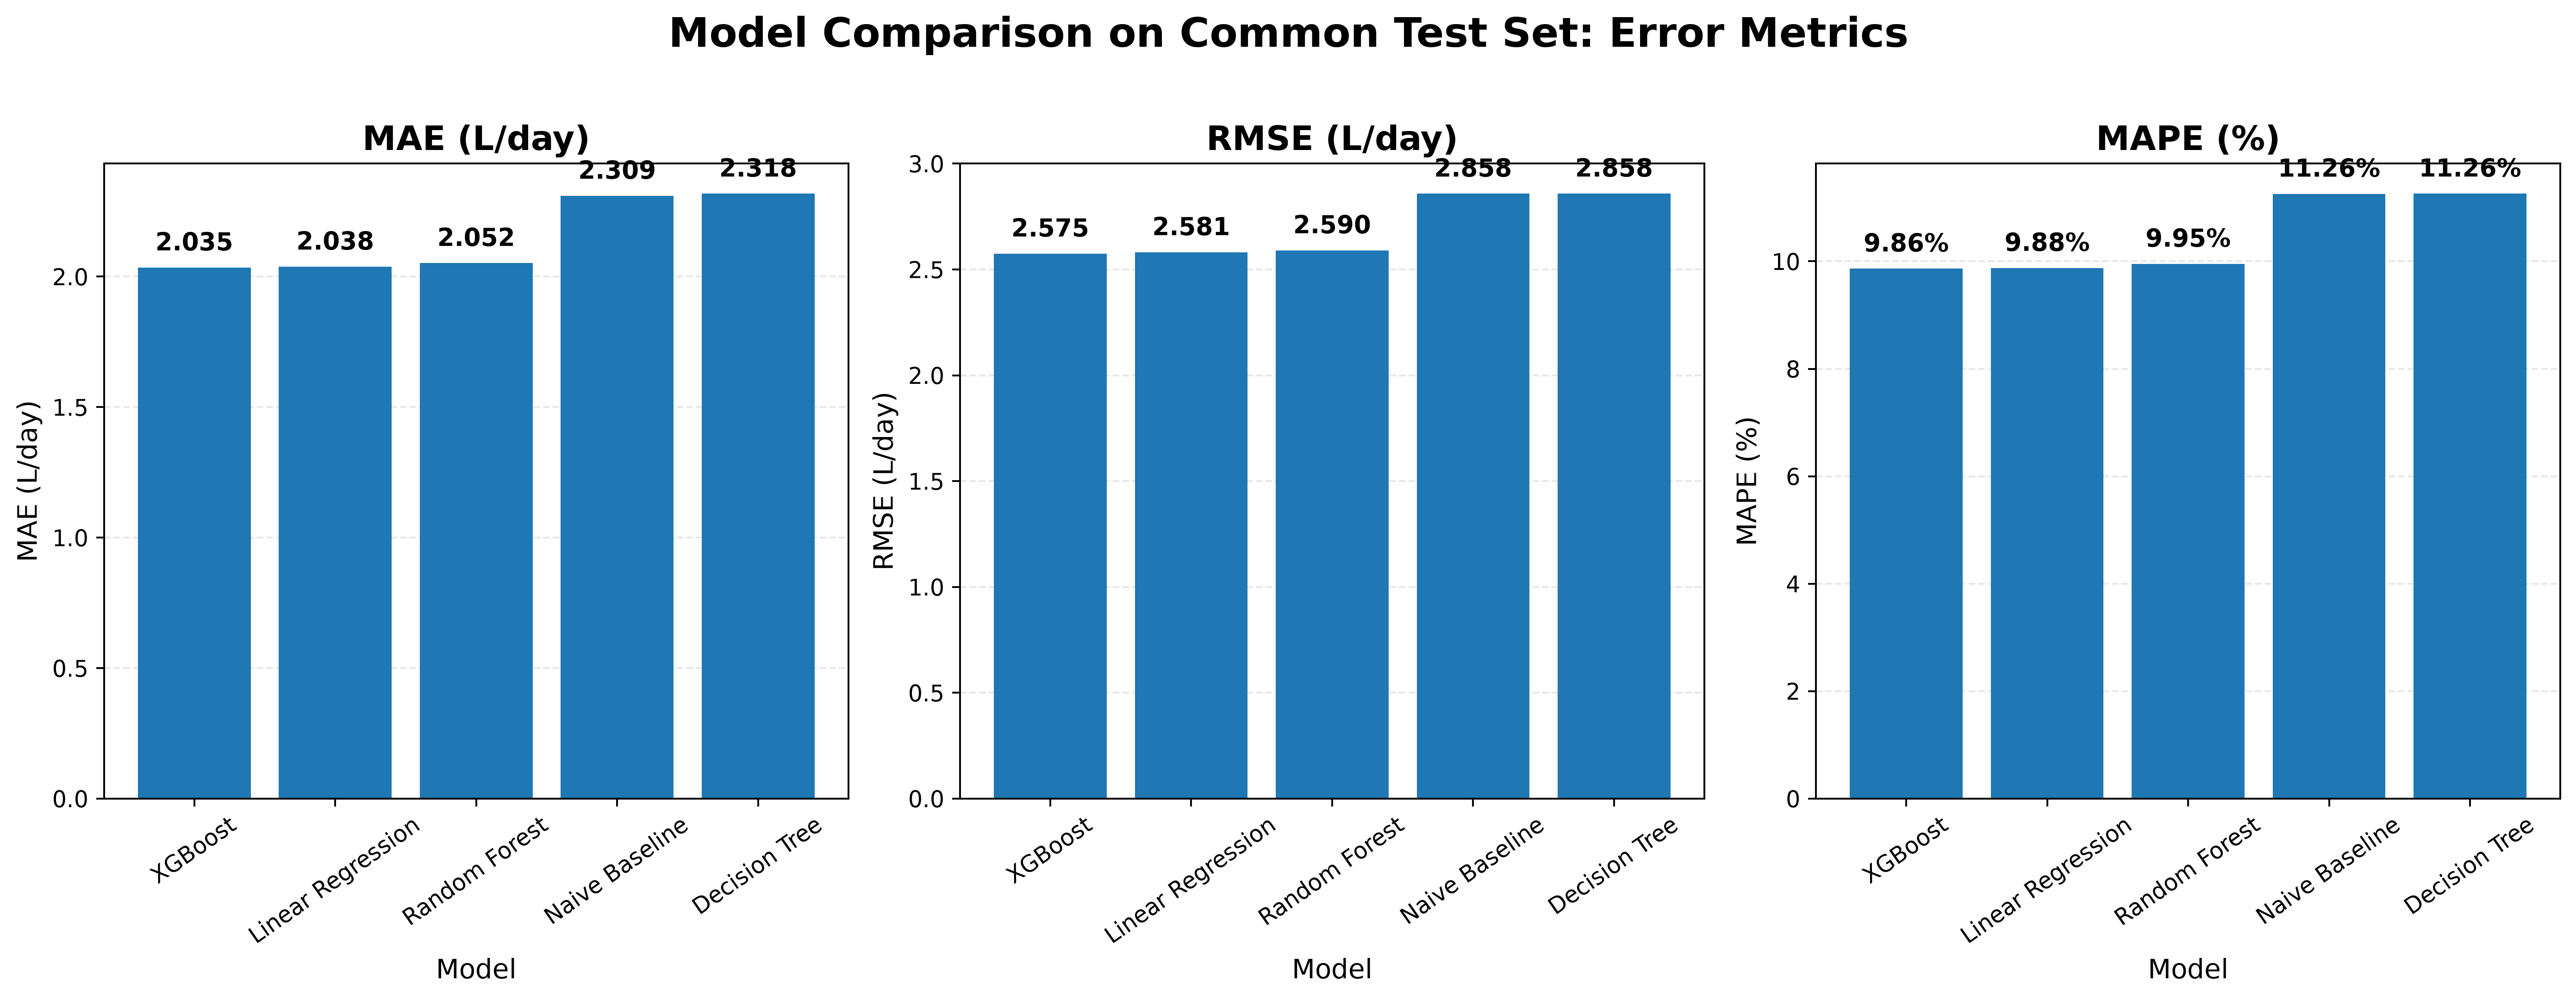
\includegraphics[width=0.95\linewidth]{../outputs/model_test_error_metrics.png}
			\caption{Test-set error metric comparison for evaluated milk-yield models on the hold-out split.}
			\label{fig:model_test_error_metrics}
		\end{figure}
		
		\begin{figure}[htbp]
			\centering
			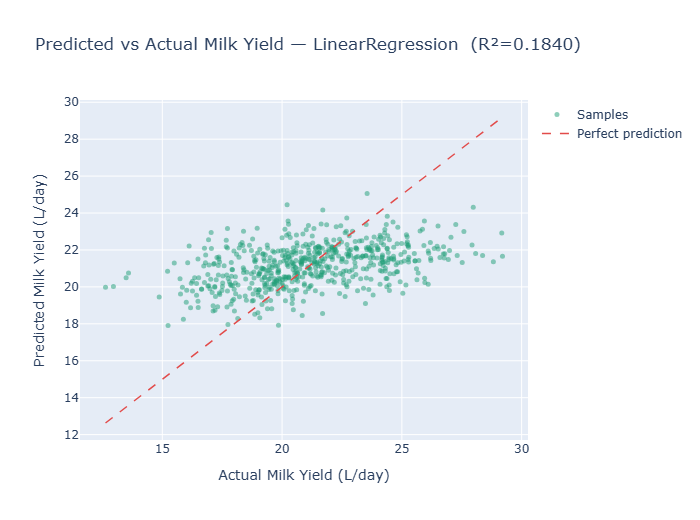
\includegraphics[width=0.95\linewidth]{../outputs/predicted_vs_actual.png}
			\caption{Predicted versus actual daily milk yield for the XGBoost model on the hold-out test set.}
			\label{fig:predicted_vs_actual_p1}
		\end{figure}
		
		\subsection{C. Explainability Analysis}
		Feature-importance and SHAP analyses were used to interpret variable contributions in the final XGBoost model. The current feature importance output indicates that body weight is the strongest global contributor, followed by age-weight ratio and weather-aware interaction terms such as temp-humidity and feed-THI interaction.
		
		\begin{figure}[htbp]
			\centering
			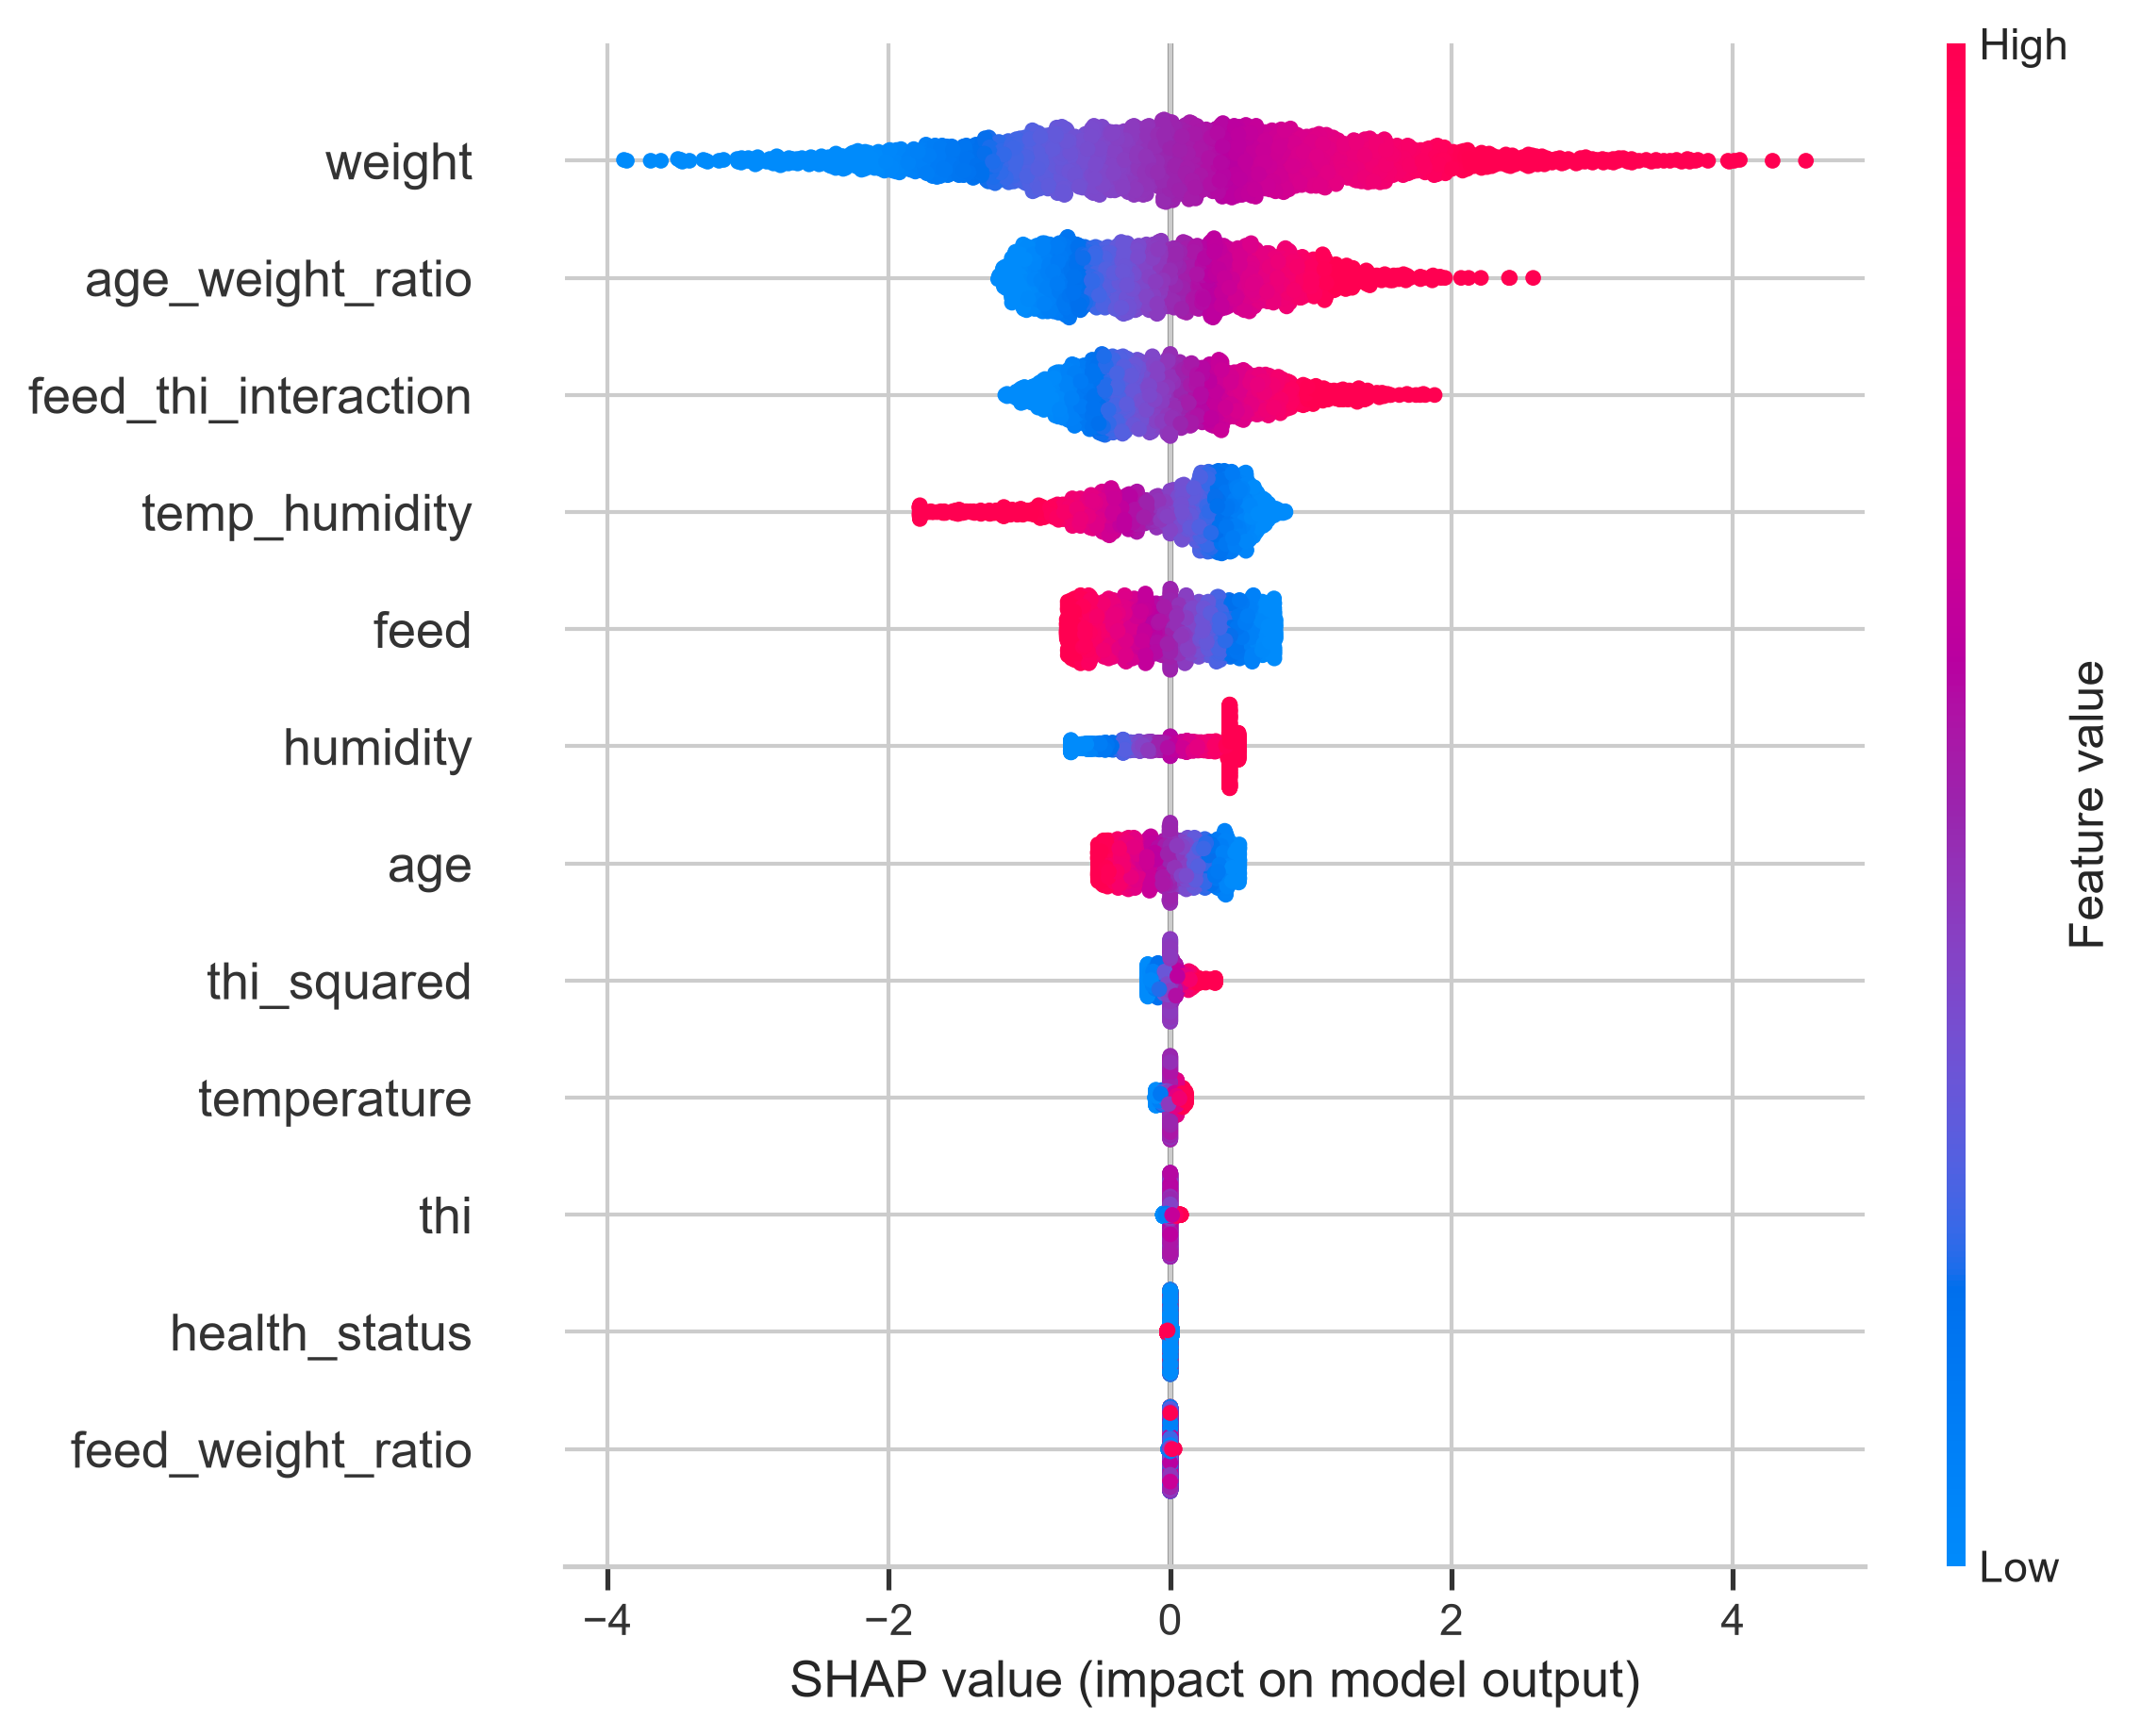
\includegraphics[width=0.95\linewidth]{../outputs/shap/shap_summary.png}
			\caption{SHAP summary plot for the final XGBoost model, showing the relative contribution of engineered weather-aware and animal variables.}
			\label{fig:shap_summary_p1}
		\end{figure}
		
		The current SHAP report confirms that weight has the largest mean absolute SHAP value (0.8996), followed by age-weight ratio (0.6806), temp-humidity (0.3992), and feed-THI interaction (0.3532). This indicates that the model depends on both biological predictors and weather-aware features in a balanced way.
		
		\subsection{D. Statistical Validation and Error Diagnostics}
		Model selection was assessed using the Wilcoxon signed-rank test on fold-wise $R^2$ scores. The current implementation reports statistically significant improvements for XGBoost relative to the other benchmark models, supporting the choice of XGBoost under the current evaluation design.
		
		Residual diagnostics also support error behavior assessment. The hold-out residuals produce a Shapiro-Wilk statistic of 0.9962 with a p-value of 0.1574, indicating that the residual distribution is not inconsistent with normality.
		
		This statistical validation confirms that the current framework is evidence-backed and keeps the analysis within the intended scope of weather-aware feature engineering and explainable milk-yield prediction.
		
		\section{Conclusion and Future Work}
		
		In this Paper 1 study, we developed and evaluated a weather-aware feature engineering framework for dairy cattle analytics and an explainable machine learning framework for milk-yield prediction with statistical validation. The current results show that XGBoost provides the best-performing model among the evaluated baselines, with a 5-fold cross-validation $R^2$ of $0.1811 \pm 0.0089$ and a hold-out test-set $R^2$ of $0.188$. The weather-aware engineered inputs, including temperature, humidity, THI, and interaction features, contribute meaningfully to the predictive framework, and the SHAP-based explainability results confirm that the model uses both biological and environmental predictors in a manner consistent with the study design.
		
		The statistical validation results further support the model choice: the Wilcoxon signed-rank tests identify significant XGBoost improvements over alternative regressors, while the Shapiro-Wilk residual test indicates that the residual distribution is not inconsistent with normality. These findings establish a clear, evidence-based Paper 1 contribution focused on weather-aware feature engineering and explainable milk-yield prediction.
		
		
		\begin{thebibliography}{00}
			\bibitem{ref1} C. A. Perez Garcia et al., ``Predicting Equivalent Temperature Index in a Cattle Barn with NeuralProphet Model,'' \textit{Agriculture}, vol. 14, no. 2, p. 316, 2024.
			\bibitem{ref2} D. B. Leal et al., ``Predicting Dry Matter Intake in Lactating Crossbred Cows Under Semi-Arid Conditions Using an Error-Based Evolving Takagi-Sugeno Fuzzy Model,'' \textit{IEEE Access}, vol. 13, pp. 71520--71529, 2025.
			\bibitem{ref3} R. Xing et al., ``Stacking Ensemble Machine Learning Modelling for Milk Yield Prediction Based on Biological Characteristics and Feeding Strategies,'' in \textit{Proc. FedCSIS}, IEEE, 2024, pp. 701--706.
			\bibitem{ref4} B. Srinithi et al., ``Enhancing Milk Yield Forecasting in Dairy Farming using an Interpretable Machine Learning Framework,'' in \textit{Proc. ICSADL-2025}, IEEE, 2025, pp. 1556--1563.
			\bibitem{ref5} W. Zhang et al., ``Daily Milk Yield Prediction of Dairy Cows Based on the GA-LSTM Algorithm,'' \textit{Comput. Electron. Agric.}, vol. 177, p. 105894, 2020.
			\bibitem{ref6} C. O'Leary and C. Lynch, ``An Evaluation of Machine Learning Approaches for Milk Volume Prediction in Ireland,'' in \textit{Proc. ISSC}, IEEE, 2022, pp. 1--8.
			\bibitem{ref7} W. J. Yan et al., ``Big Data Analytics for Empowering Milk Yield Prediction in Dairy Supply Chains,'' in \textit{Proc. IEEE Big Data}, IEEE, 2016, pp. 2131--2137.
			\bibitem{ref8} M. B. Prasad, ``Regression for Forecasting Meat Production Using Milk Data,'' \textit{IEEE/ACM Trans. Comput. Biol. Bioinform.}, vol. 21, pp. 150--162, 2024.
			\bibitem{ref9} G. Thangarasu and K. R. Alla, ``Optimization of Livestock Farming Using Multi-Tasking Regularisation Model,'' in \textit{Proc. SmartTechCon}, IEEE, 2023, pp. 945--950.
			\bibitem{ref10} Z. Z. Feng et al., ``The LASSO and Sparse Least Squares Regression Methods for SNP Selection in Predicting Quantitative Traits,'' \textit{IEEE/ACM Trans. Comput. Biol. Bioinform.}, vol. 9, no. 2, pp. 628--636, 2012.
			\bibitem{ref11} S. Yadav, ``Livestock Health Monitoring Using Multisensor Data and Machine Learning Techniques,'' \textit{Eng. Appl. Livestock Prod.}, vol. 6, pp. 1--6, 2025.
			\bibitem{ref12} W. M. C. S. Bandara et al., ``Machine Learning and Image Processing Based Approach for Improving Milk Production and Cattle Livestock Management,'' in \textit{Proc. ICCCNT}, IEEE, 2022, pp. 1--6.
			\bibitem{ref13} S. I. Arafat et al., ``Real Time Cattle Health Monitoring and Early Disease Detection Using IoT and Machine Learning,'' in \textit{Proc. ICESC}, IEEE, 2024, pp. 455--460.
			\bibitem{ref14} R. J. Michelle et al., ``Edge AI enabled IoT System for Cattle Behavior Monitoring and Classification,'' \textit{Inf. Process. Agric.}, vol. 12, pp. 42--51, 2025.
			\bibitem{ref15} J. Umamageswaran et al., ``A Hybrid Sensor--Image Framework for Smart Farming Using Deep and Ensemble Learning,'' in \textit{Proc. AI Summit}, IEEE, 2025, pp. 1--6.
			\bibitem{ref16} R. Chaudhary and S. Gupta, ``Challenges in Milk Yield Forecasting and Feed Optimization: A Comparative Study of AI-Based and Quantum-Enhanced Dairy Systems,'' \textit{Comput. Electron. Agric.}, vol. 219, p. 108734, 2024.
			\bibitem{ref17} Z. Fan, ``Construction of Food Quality Prediction and Traceability Platform Based on Machine Learning,'' in \textit{Proc. WCONF}, IEEE, 2025, pp. 1--7.
			\bibitem{ref18} M. Molins et al., ``Non-Invasive Thermal Monitoring of Dairy Cows' Core Body Temperature with Multi-Modal Sensing,'' in \textit{Proc. IEEE PLF}, IEEE, 2025, pp. 455--460.
			\bibitem{ref19} S. Seema and L. Ramesh, ``An Explainable AI Framework Combining Multi-Task GCN and Reinforcement Learning for Adaptive Feeding and Animal Health Management in Dairy Farming,'' in \textit{Proc. ICSCN}, IEEE, 2025, pp. 1261--1268.
			\bibitem{ref20} N. Hoggas et al., ``Advancing Milk Quality Prediction: Dynamic Stacking Ensemble with Quality-Aware Adaptive Sampling,'' in \textit{Proc. ICAAID}, IEEE, 2025, pp. 1--7.
		\end{thebibliography}
		
\end{document}
